%!TEX root = ../Main.tex

\chapter[expVIP]{expVIP: a customisable RNA-seq data analysis and visualisation platform}
\label{cha:exp}

\section{Background.}
Describe the list of previously published expression experiments and how they can potentially be used as a framework for new experiments.  

Co-expression of homoeologus varies from triplet to triplet \citep{Pfeifer2014}
The silencing is mostly regulated by epigenetic changes as the hybridization events are recent.  \citep{Bottley2006}

Kallisto vs sailfish vs tuxedo. 

Table of experiments to include 

The software developed in this section is published in \citep{Borrill2016}. 

\subsection{Relational databases}
A Relational databases is a set of structured tables that have relationships between each other. 
The tables correspond to the data that is essential for the represented concept (domain).
For example, in a table representing several species, the common name and the scientific name belong to the same domain (ie name: Bread wheat; scientific name \textit{Triticum aestivum}). 
Tables in the same relational database form relationships between each other. 
Continuing with the example, an species can have several scientific studies related to them. 
The domain of a study can be formed by the accession, a title, a corresponding manuscript and the species that concerns to it. 
A set of columns that have unique values across the table is called a primary key, in our example an extra \texttt{id} column is added (Figure \ref{fig:expvip:miniER}; \citealt{Codd1970}).
The tables \ref{exp:tab:species} and \ref{exp:tab:studies} have the content of their corresponding domains. 

\begin{figure}
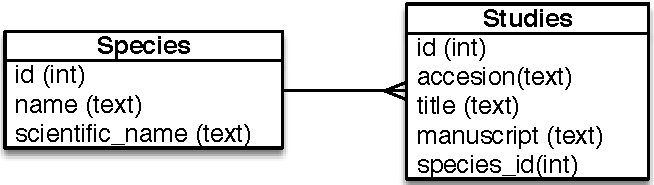
\includegraphics{expVIP/Figures/miniER.pdf}
\caption[Example of a relationship between table.]{Example of a relationship between table. The tables Species and Studies are related. Each study has one species and each species can have several studies.}
\label{fig:expvip:miniER}
\end{figure}

\begin{table}
\caption[Species]{Example content for the table \texttt{species}}
\label{exp:tab:species}
\centering
\begin{tabular}{rll}
\toprule
   id & name                          & scientific\_name                                         \\
\midrule
    1 & Bread wheat                 & Triticum aestivum                                     \\
    2 & Yellow rust                 & Puccinia striiformis              \\
    3 & wheat and rust & T.aestivum,S.tritici  \\
\bottomrule
\end{tabular}

\end{table}

\begin{table}
\caption[Studies]{Example content for the table \texttt{studies}}
\label{exp:tab:studies}
\centering
\begin{tabular}{rllr}
\toprule
   id & accession                                          & manuscript                              &   species\_id \\
\midrule
    1 & DRP000768                                          &  10.1186/1471-2164-14-77          &            1 \\
    2 & ERP003465                                          & 10.1186/1471-2164-14-728            &            1 \\
    3 & ERP004505                                          &  10.1126/science.1250091          &            1 \\
    4 & SRP004884                                          & 10.1186/1471-2164-12-492            &            1 \\
    5 & SRP013449                                          &  10.1111/j.1467-7652.2012.00705.x &            1 \\
    6 & SRP017303                                          & 10.1186/1471-2164-14-270            &            2 \\
    7 & SRP022869                                          &  10.1371/journal.pone.0081606     &            3 \\
\bottomrule
\end{tabular}

\end{table}

\subsection{SQL}
\gls{sql} is a common language to retrieve information from relational databases. 
\acrshort{sql} has operations to select columns and row, join tables, group repeated values and order the results. 
Those simple operations are enough to retrieve the information between tables \citep{Oracle2014}. 
The following list shows a brief description of some commands build a query.  

\begin{description}
\item[\texttt{SELECT <EXPRESSIONS> }]. A list of columns or an expression that will be displayed, separated by commas (\texttt{,}). To display all the columns, the \texttt{*} character represents all the tables. The order of the columns will be the same as the order given in this part of the command
\item[\texttt{FROM <TABLE>}]. follows the column names to add a list of tables to select.
\item[\texttt{JOIN <TABLE> ON <EXPRESSION> }]. is used to join the table from the left side of the statement with the \texttt{<EXPRESSION>} given after the \texttt{ON} clause.  
\item[\texttt{WHERE <EXPRESSION>}] filters the rows by the \texttt{<EXPRESSION>}
\item[\texttt{ORDER BY <COLUMNS>}]. The rows will be sorted by the natural order of the given \texttt{<COLUMNS>}.  
\item[\texttt{GROUP BY <COLUMNS>}]. The rows are merged by the columns stated. This can be used to get an unique set of values and apply a function to all the rows that have the same value, as a count.
\end{description} 

Expressions can be values, operators or functions like:

\begin{description}
\item[\texttt{COLUMN}] The value of a column. 
\item[ \texttt{<EXPRESSION> = <EXPRESSION>}] \texttt{TRUE} when the left and right \texttt{<EXPRESSION>} are equal. \texttt{FALSE} otherwise 
\item[ \texttt{<EXPRESSION> > <EXPRESSION>}] \texttt{TRUE} when the left  \texttt{<EXPRESSION>} is greater than the  right \texttt{<EXPRESSION>} are equal. \texttt{FALSE} otherwise 
\item[ \texttt{<EXPRESSION> < <EXPRESSION>}] \texttt{TRUE} when the left  \texttt{<EXPRESSION>} is less than the  right \texttt{<EXPRESSION>} are equal. \texttt{FALSE} otherwise
\item[ \texttt{COUNT(*)}] The count of rows that have the same values, as selected in the \texttt{GROUP BY} clause.
\end{description}

A simple query to join the  \texttt{species} and \texttt{studies} tables and displaying only the species name, scientific name and accession of the study is shown in Listing \ref{exp:lst:joinExample}. 
The results of the query are in Table \ref{exp:tab:joinExample}. 

\begin{code}[language=sql, label=exp:lst:joinExample,caption=Join example query]
SELECT 
	species.name, 
	species.scientific_name, 
	studies.accession, 
FROM species
JOIN studies on species.id = studies.species_id;
\end{code}

\begin{table}[h!]

\caption[Join example]{Join of the \texttt{species} and \texttt{studies} table. }
\label{exp:tab:joinExample}
\centering
\begin{tabular}{lll}
\toprule
 name                          & scientific\_name                                         & accession                                                                       \\
\midrule
 Bread wheat                 & Triticum aestivum                                     & DRP000768                                          \\ 
 Bread wheat                 & Triticum aestivum                                     & ERP003465                                          \\ 
 Bread wheat                 & Triticum aestivum                                     & ERP004505                                          \\ 
 Bread wheat                 & Triticum aestivum                                     & SRP004884                                          \\ 
 Bread wheat                 & Triticum aestivum                                     & SRP013449                                          \\ 
 Yellow rust                 & Puccinia striiformis            & SRP017303                                          \\ 
 wheat and rust & T.aestivum,S.tritici & SRP022869                                          \\ 
\bottomrule
\end{tabular}

\end{table}


The relationships between tables can be of the following types:

\begin{description}
\item[one-to-one] When rows on a table can be related to a row in a second table. On the diagrams they are represented by a straight line
\item[many-to-many] Rows on a table can have many corresponding rows in a second table, resented with lines with whiskers on both sides of the line.  
\item[one-to-many] Rows on a table can be related to many rows on the second table, represented with whiskers only on one side of the line. 
\end{description}

An important feature of a database is the ability to store the 
data consistently.
A transaction is a set of related operations that need to be performed at the same time.  
To ensure that a transaction needs to follow the principles of \gls{acid} \citep{Haerder1983}.


\begin{description}
\item[Atomicity.] All the operation or none have to be performed. If any of them fails or an error happens while the transaction is executed the data has to be restored to the original status before the transaction started. 
\item[Consistency.] The changes in the database have to be valid before and after the transaction. 
\item[Isolation.] If more than one transaction is being executed at the same time, the result must be the same as if the transactions were executed one after the other. 
\item[Durability.] The result of the transaction is stored even if the server is restarted.
\end{description}  

Several \gls{rdbms} implement \acrshort{sql}, with various levels of compliance to the standard and different licenses.  
A popular \acrshort{rdbms} is \texttt{MySQL}.
From the beginning \texttt{MySQL} aimed to be a lightweight and easy to install open source product \citep{Oracle2014}. 
This characteristics made it popular on the web and it is currently the \gls{rdbms} behind ensembl! \citep{Flicek2012}. 

\subsection{Model-View-Controller}

\begin{SCfigure} 
  \centering
  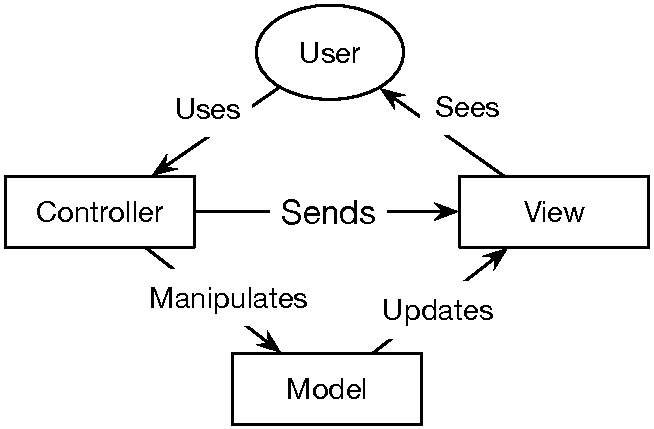
\includegraphics[width=0.7\textwidth]{LitReview/Figures/MVC.pdf}
  \caption{\acrshort{mvc} interaction between components.}
  \label{fig:poly:mvc}
\end{SCfigure}
The \gls{mvc} is a metaphor to isolate the user interactions from the underlying data. 
The models hold the data on logical their domains.
The views contain the layout on how the models are displayed to the user.
The controllers receive the requests from the users and modify the models accordingly and send a view back for display. 
The \acrshort{mvc} metaphor allows the development of independent parts of the system and helps to structure the underlying representation of the domains.  (Figure \ref{fig:poly:mvc}; \citealt{Krasner1988}).

\gls{ror} is a framework to develop web applications heavily influenced by the \acrshort{mvc} metaphor. 
It is based on the Rails language and provides several tasks designed to facilitate the development, such as automated tasks designed to create models with their corresponding views and controllers. 
On the top of that, it provides the tools to manage the connection and queries to the \acrshort{rdbms}, allowing the developer to focus on the functionality \citep{RailsGuide2016}. 

\subsection{Aims}

The aims of expVIP are to:
\begin{enumerate}
\item Integrate RNA-Seq experiments from several sources in a single database (Section \ref{exp:DB}). 
\item Automate the calculation of the expression values and load them in to the database (Section \ref{exp:pipeline}).
\item Produce a visualization for said expression values (Section \ref{exp:gui}).
\item Make the system available to the community (Section \ref{exp:gui}).
\end{enumerate}


\section{General design}

One of the main objectives of expVIP is to make the public expression datasets to the target community (currently wheat, but not limited to it). 
A web interface is an effective is an effective way to reach a global audience. 
A web service requires to have a server to run the application and a browser to connect to the server and display it (ie Internet Explorer, Chrome).
The web server technology used for expVIP is \acrshort{ror}, as it abstracts the \acrshort{mvc} metaphor and it is designed to speed the development \citep{RailsGuide2016}. 
In order to display the expression data to the users, a BioJS component (\citealt{Yachdav2015}, Section \ref{exp:gui}). 
All the data is stored in a MySQL database (Section \ref{exp:DB}) and it is accessed trough models developed under  \acrshort{ror} (Figure \ref{fig:poly:archDesign}).  

\begin{figure} 
  \centering
  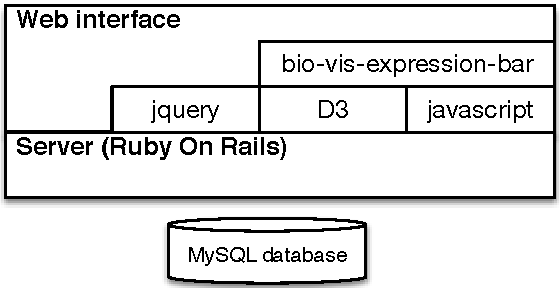
\includegraphics[width=0.9\textwidth]{expVIP/Figures/archDesign.pdf}
  \caption{General design of expVIP}.
  \label{fig:poly:archDesign}
\end{figure}

\section{Database design} 
\label{exp:DB}

To address the different types of conditions over different experiments, expVIP is designed around a relational database. 
The design comprises of two core groups of tables and two auxiliary tables that take care of different species and  homoeologues and (Figure \ref{fig:expvip:dbDesign}).


\begin{sidewaysfigure}
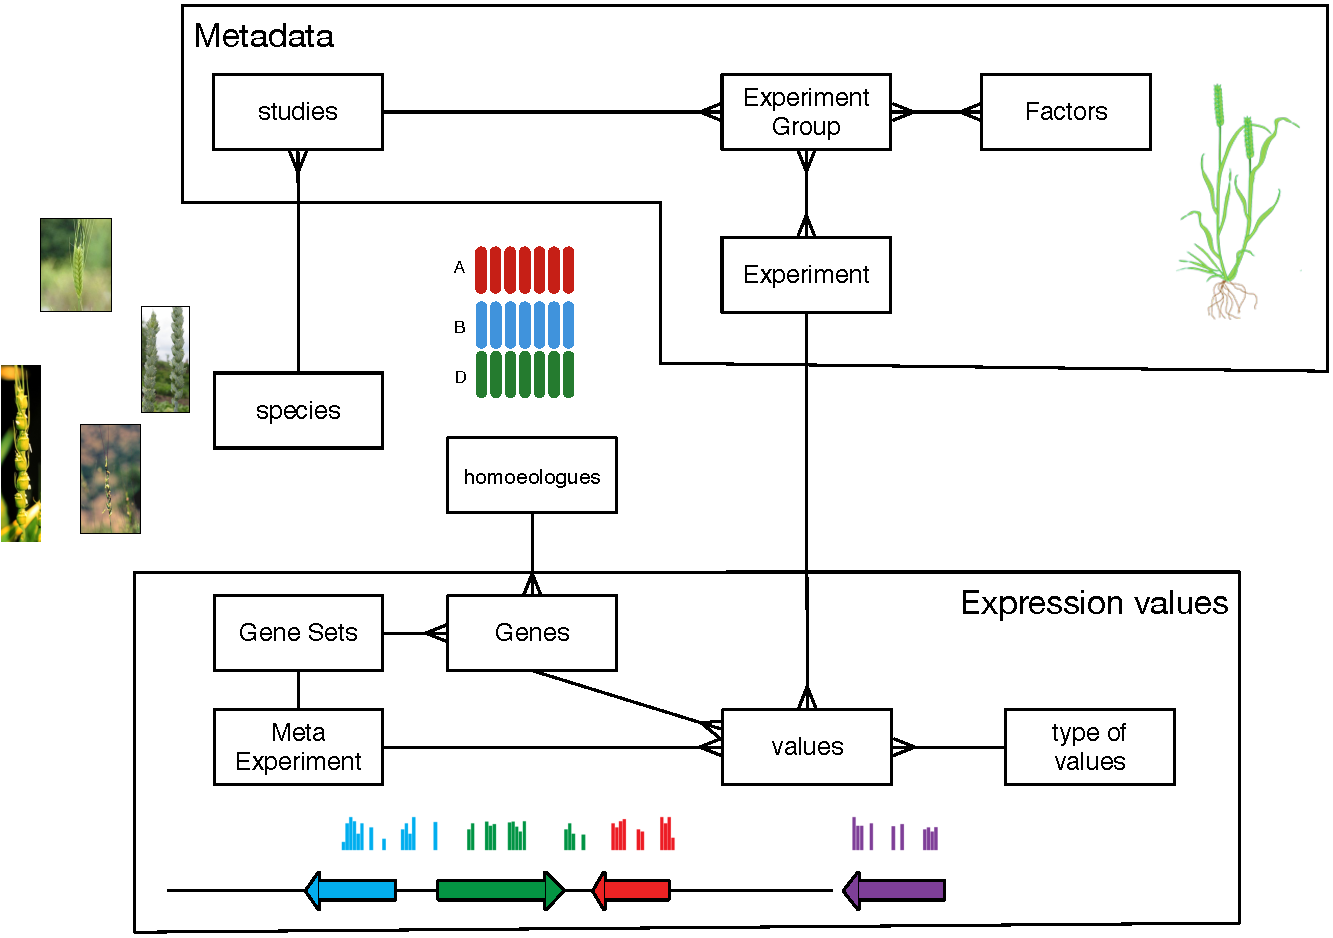
\includegraphics[width=1\textheight]{expVIP/Figures/dbDesign.pdf}
\caption[expVIP database design]{Database design. The block on the top stores the meta-data about the experiments and the studies. The bottom block consist on the tables related to the expression values. Species and homoeologues are outside the main blocks as they are not core to the groups. The whiskers in the connections show the cardinality of the relationships.  }
\label{fig:expvip:dbDesign}
\end{sidewaysfigure}

\begin{description}
\item[Metadata] The tables in this group contain the information of each one of the studies. 
\begin{description}
\item[Studies] Contains the general information of a study, which contain several experiments. The table also contains the reference to the paper where the data is published and the accession for the study. 
\item[Experiment group] keeps together all the individual experiments that come from the same study and that were taken on the same condition (ie. replicates). 
\item[Factors] holds all the possible factors used to group the experiments. Each experiment group has many factors and each factor group has many experiment groups. As the experiment doesn't have a fixed number of column representing each factor, it is possible to have any arbitrary number factors to group. 
\item[Experiment] holds the information of each individual experiment, with the corresponding accession. 
\end{description}
\item[Expression values.] The tables on this block contain the expression of each gene and the information for the genes. 
\begin{description}
\item[Types of value] keeps a list of different units that are stored. On the original design \acrshort{tpm} and raw counts are set up, but as the units are not hard coded it is possible to use \acrshort{fpkm}, \acrshort{rpkm} or, any other unit. 
\item[Gene Set] contains the name of a reference gene set for the analysis. On the original version of expVIP, the gene models from the \acrshort{iwgsc} as deposited in Ensembl release 26 were used \citep{Mayer2014} However, the use of this table enable the use of several reference gene models on the same database. 
\item[Genes] are related to a \texttt{gene set}, so even if they have the same name coming from different datasets it is possible to distinguish them. This situation is unlikely to occur when using published references, but when joining several \textit{de Novo} gene models. 
\item[Meta Experiment] allows to have the same data analysed with different tools. By default expVIP uses Kallisto \citep{Bray2016}. However other tools, or different versions of the same tool, can be used to repeat the analysis.   
\item[Values] have a domain that includes the \texttt{meta experiment}, \texttt{gene} and, \texttt{type of value}.
\end{description}
\item[Homoeologues] contain the relationship between genes. This allows to get the expression values of several related genes. 
\item[Species] contain the target species of a study. It is not linked to the gene models to allow the direct comparison between related species using the same gene models (ie, \texttt{T. aestivum} vs \texttt{T. turgidum}). 
\end{description}

In the cases that a relationship between tables is not unique, such as \texttt{experiment\_groups} having many \texttt{factors} and the \texttt{factors} having many \texttt{experiment\_groups}, storing the relationships is done with an auxiliary table (ie. \texttt{ExperimentGroups\_Factors}, not explicitly shown in Figure \ref{fig:expvip:dbDesign}, but implicit by the lines with whiskers). 

%The database is designed to be flexible to accommodate users using non-model organisms were the available resources may be limited. 

Once all the data is stored, the tables can be queried together to make clear the relationship between specific rows. 
One of the core tasks of expVIP is to get all the factors that define each experiment, in order to be able to merge similar studies. 
To retrieve the \texttt{experiments} and \texttt{factors} of an \texttt{experiment group}, the auxiliary tables \texttt{ExperimentGroups\_Factors}  and \texttt{experiment\_groups\_experiments} are used in the query. (Listing \ref{lst:exp:queryMetadata} and Table \ref{tab:exp:queryMetadata}).


\begin{code}[language=sql, caption={[Query experiments and factors]Query experiments and factorsQuery experiments and factors from accession 'DRR003148'},label=lst:exp:queryMetadata]
SELECT
	experiments.accession,  
	factors.factor,
	factors.description, 
	experiment_groups.name as expriment_group 
FROM factors 
JOIN ExperimentGroups_Factors 
	ON factors.id = ExperimentGroups_Factors.factor_id
JOIN experiment_groups 
	ON experiment_groups.id = ExperimentGroups_Factors.experiment_group_id
JOIN experiment_groups_experiments 
	ON experiment_groups_experiments.experiment_group_id = experiment_groups.id
JOIN experiments 
	ON experiments.id = experiment_groups_experiments.experiment_id
WHERE accession =  'DRR003148'
\end{code}

%\pagebreak
\begin{table}[h]
\caption[Results of query for metadata]{Results of querying the metadata for accession 'DRR003148' (Listing \ref{lst:exp:queryMetadata})}
\label{tab:exp:queryMetadata}
\begin{tabular}{llll}
\toprule
 accession   & factor                    & description    & expriment   \\
     &                     &     & group   \\
\midrule
 DRR003148   & Age                       & 24 days        & Group1            \\
 DRR003148   & High level age            & vegetative     & Group1            \\
 DRR003148   & High level stress-disease & no stress      & Group1            \\
 DRR003148   & High level tissue         & roots          & Group1            \\
 DRR003148   & High level variety        & Chinese Spring & Group1            \\
 DRR003148   & Stress-disease            & none           & Group1            \\
 DRR003148   & Tissue                    & roots          & Group1            \\
 DRR003148   & Variety                   & Chinese Spring & Group1            \\
\bottomrule
\end{tabular}

\end{table}

Likewise, to get the \texttt{expression\_values} for a \texttt{gene} with the corresponding unit (\texttt{type\_of\_values}) and \texttt{experiment} a simple query joining the four tables is used. 
The Listing \ref{lst:exp:queryExpValues} retrieves the \texttt{expression\_values} for the \texttt{gene} 'Traes\_5BS\_0AFC3F795.1', and the result is on Listing \ref{tab:exp:queryExpValues}

\begin{code}[language=sql, caption={[Query values for gene and experiment group] Query values from 'Group1' and gene 'Traes\_5BS\_0AFC3F795.1' },label=lst:exp:queryExpValues]
SELECT 
	genes.name as gene, 
	expression_values.value,
	experiments.accession,
	type_of_values.name as unit
FROM expression_values
JOIN genes 
	ON expression_values.gene_id = genes.id
JOIN type_of_values 
	ON type_of_values.id = expression_values.type_of_value_id
JOIN experiments 
	ON experiments.id = expression_values.experiment_id
WHERE 
	genes.name = 'Traes_5BS_0AFC3F795.1' 
\end{code}

\begin{table}[h]
\caption[Results of query for values]{Results of query to get the values for gene 'Traes\_5BS\_0AFC3F795.1' (Listing \ref{lst:exp:queryExpValues}), only 'Group1' is displayed from the output.}
\label{tab:exp:queryExpValues}
\begin{tabular}{lrlll}
\toprule
 gene                  &    value & accession   & experiment   & unit   \\
                    &     &    & group   &    \\
\midrule
 Traes\_5BS\_0AFC3F795.1 & 136.995  & DRR003148   & Group1             & count  \\
 Traes\_5BS\_0AFC3F795.1 & 120.683  & DRR003149   & Group1             & count  \\
 Traes\_5BS\_0AFC3F795.1 & 140.94   & DRR003150   & Group1             & count  \\
 Traes\_5BS\_0AFC3F795.1 &  24.2277 & DRR003148   & Group1             & tpm    \\
 Traes\_5BS\_0AFC3F795.1 &  23.9739 & DRR003149   & Group1             & tpm    \\
 Traes\_5BS\_0AFC3F795.1 &  24.9835 & DRR003150   & Group1             & tpm    \\
\bottomrule
\end{tabular}

\end{table}

With those two queries is enough to retrieve all the information required to do sub-groupings. 

The database is implemented using the \acrshort{rdbms} \texttt{MySQL 5.5}. 



\section{Data integration pipeline} 
\label{exp:pipeline}


To prepare the database, expVIP requires to have all the metadata for the experiments to integrate. 
ExpVIP contains tasks to load all the metadata and a wrapper for Kallisto that can be run from expVIP. 
Alternatively, the expression values can be calculated with another tool and loaded as a single file, this approach is preferred for a large set of samples (Figure \ref{fig:exp:loadPipeline}). 
Details on how to load the files in the database are in the expVIP tutorial (Appendix \ref{exp:tutorial}). 

\begin{figure}
\centering
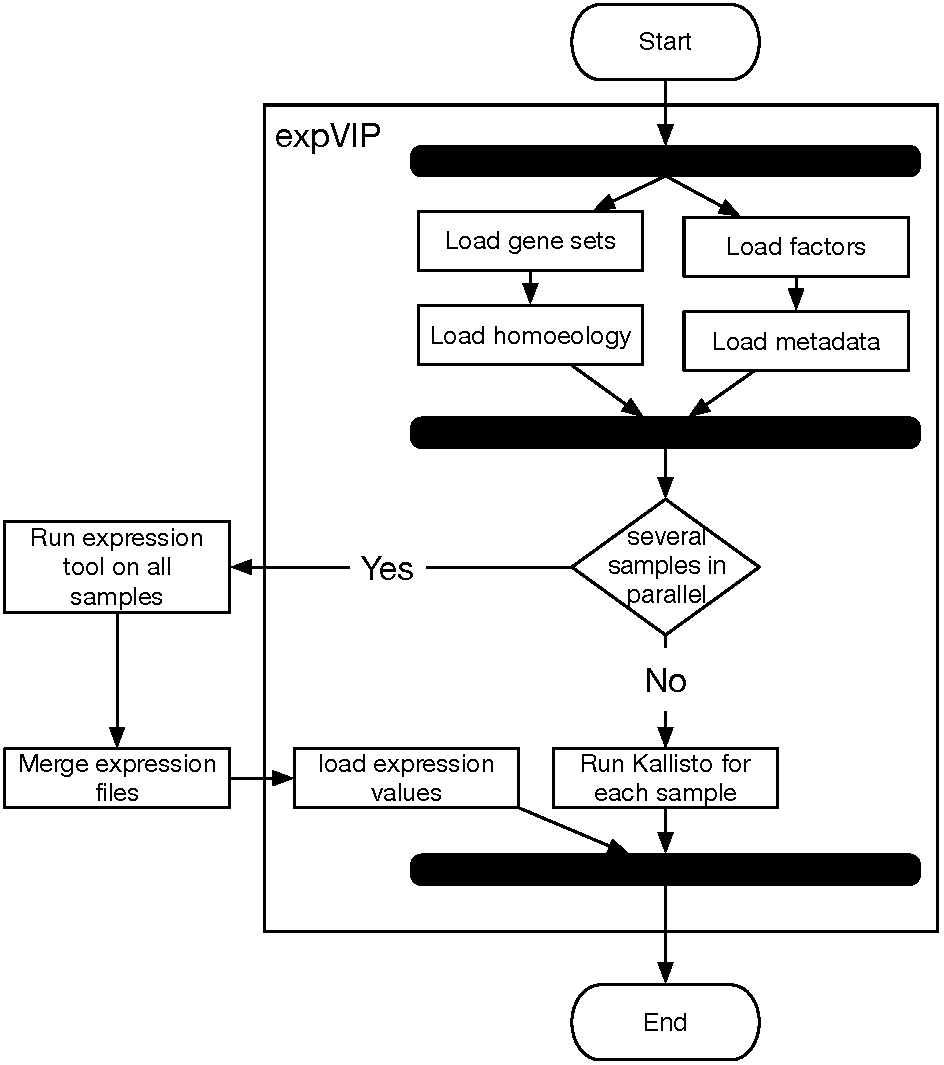
\includegraphics[width=1\textwidth]{expVIP/Figures/loadDataPipeline.pdf}
\caption[expVIP load data]{The pipeline of loading the data to expVIP. The black lines represent a border of tasks that can be run in parallel or don't require to be done in a particular order.}
\label{fig:exp:loadPipeline}
\end{figure}

The required files for the metadata are:
\begin{description}
\item[Factors.] The file contains all the possible factors that can be used to group all the experiments. The file must contain the following columns (Table \ref{tab:exp:factors}):
\begin{description}
\item[factor] The category were the factor belongs. In the case of the initial dataset used in expVIP, the grouping factors are: Age, stress-disease, tissue and, a corresponding 'High level' for each factor. The metadata file must contain a cloumn corresponding to each one of this factors. 
\item[order] The default order in which to display each factor. This ensures that the age of the plants are sorted chronologically. 
\item[name] Long description of each factor. This are used as valid values in the metadata.  
\item[short] Is a short name, used when the space to display the full description of the factor is not enough.
\end{description}
\begin{table}
\centering
\caption[Factors file]{Factors file. The table must be saved as a text file, with columns separated by tabs}
\label{tab:exp:factors}
\begin{tabular}{llll}
\toprule
factor & order & name & short \\
\midrule
Age & 1 & 7 days & 7d \\
Age & 2 & seedling stage & see \\
Age & 3 & 14 days & 14d \\
Age & 4 & three leaf stage & 3\_lea \\
Age & 5 & 24 days & 24d \\
High level age & 1 & seedling & see \\
High level age & 2 & vegetative & veg \\
High level age & 3 & reproductive & repr \\
High level stress-disease & 1 & none & none \\
High level stress-disease & 2 & disease & dis \\
High level stress-disease & 3 & abiotic & abio \\
High level stress-disease & 4 & transgenic & trans \\
High level tissue & 1 & spike & spike \\
High level tissue & 2 & grain & grain \\
... & & \\
\bottomrule
\end{tabular}
\end{table}
\item[metadata] The metadata file is the file that contains the information related to each study and the corresponding experiments. 
Each study contains several experiment groups (replicates), which in turn contain every individual experiment. 
The factors must be shared across experimental groups. 
\begin{description}
\item[secondary\_study\_accession] The accession number for experiments carried as part of a single study. This is usually the high level BioProject or SRA number. 
\item[run\_accession] The accession of the individual run. 
\item[scientific\_name] of the species. 
\item[experiment\_title] A description for the individual RNA-seq sample.
\item[study\_title] A description of the general study.
\item[Manuscript] The DOI of the study.
\item[Group\_for\_averaging] A description of the experiment. This must be the same all the replicates in the same study. 
\item[Group\_number\_for\_averaging] A short name for replicated experiments.  
\item[Total reads] (optional)
\item[Mapped reads] (optional)
\end{description}
Besides the main fields, each factor has a a corresponding column Variety, Tissue,Age, Stress-disease, High level variety, High level tissue, High level age and, High level stress-disease

\item[Gene set] The gene set is provided as a single fasta file. 
The file may contain alternative transcripts from the same gene. To identify this, the fasta header may include the optional fields \texttt{gene} and \texttt{transcript}. 
On the absence of this, the only stored value is the name from the \textgreater  character to the first space (Listing \ref{lst:poly:geneFa}). 

\begin{code}[label=lst:poly:geneFa, caption={[Gene set fasta file] A fasta entry on of the gene set.}]
>Traes_5BL_3FC5BA305.1 cdna:novel scaffold:IWGSC2:IWGSC_CSS_5BL_scaff_1082268:5:199:-1 gene:Traes_5BL_3FC5BA305 transcript:Traes_5BL_3FC5BA305.1
TGCTGCTGCTAGGCTTGAAGAGGTTGCTGGCAAGCTCCAGTCTGCTC
GGCAGCTCATTCAGAGGGGCTGTGAGGAGTGCCCCAAGAACGAGGAT
GTTTGGTTCGAGGCATGCCGGTTGGCTAGCCCAGATGAGTCAAAGGC
AGTAATTGCCAGGGGTGTGAAGGCAATTCCCAACTCTGTGAAGCTGT
GGCTGCA
\end{code}
\item[homoeologues] A file containing the homoeologues for the  A, B and D genomes. Currently this are the only supported default names. The file also include a column with the gene name and to which Group (ie 1, 2, 3 ... 7) and Genome (ie A, B or D) it belongs (Table \ref{tab:exp:hom}).  

\begin{sidewaystable}
\centering
\caption[Homoeology file]{Example tabular file containing the homoeology across the three genomes. }
\label{tab:exp:hom}
\begin{tabular}{llllll}
\toprule
Gene & A & B & D & Group & Genome \\
\midrule
Traes\_5BS\_0AFC3F795 & Traes\_5BS\_0AFC3F795 & Traes\_5BS\_0AFC3F795 & Traes\_5DS\_C204EBAA9 & 5 & B \\
Traes\_5DS\_C204EBAA9 & Traes\_5DS\_C204EBAA9 & Traes\_5BS\_0AFC3F795 & Traes\_5DS\_C204EBAA9 & 5 & D \\
Traes\_7DL\_82360D4EE1 & Traes\_7DL\_82360D4EE1 & Traes\_7DL\_82360D4EE1 & & 7 & D \\
Traes\_2AL\_1368BE0AD & & Traes\_2AL\_1368BE0AD & Traes\_2BL\_CD459994C1 & 2 & A \\
... & & & & &  \\
\bottomrule 
\end{tabular}
\end{sidewaystable}
\end{description} 

expVIP includes several tasks to load the different files. 
For example, to load the factors the \verb|load_data:factor| starts a transaction (Listing \ref{lst:exp:laodFactor}; line 2) to ensure that all the data is loaded, and if for some reason the load fails, the database is restored to the previous status.
In the transaction, the file is open with the \verb|csv| library row by row (line 3).
The function \verb|find_or_create_by| is a function that \acrshort{ror} provides on models to create an entry in the table, or update it if already exists.
Each row is used to create or update a \verb|Factor| (lines 374-376). 
A similar strategy is used for all the files that are regular tables. 

\begin{code}[language=ruby, caption={[Load factors]Task that loads factors}, label=lst:exp:laodFactor]
task :factor, [:filename] => :environment do |t, args|
  ActiveRecord::Base.transaction do 
    CSV.foreach(args[:filename], :headers => true, :col_sep => "\t") do |row|
      factor = Factor.find_or_create_by(:factor=>row["factor"],  :description=>row["name"],  :name=>row["short"])
      factor.order = row["order"].to_i
      factor.save!
    end
  end
end
\end{code}

The gene sets are loaded slightly differently, as the input is a \verb|fasta| file, as opposed to tabular file. 
The reader for the \verb|FastaFormat| from BioRuby \citep{Goto2010} is used to read the file (Listing \ref{lst:exp:loadGenes}; line 4). 
Since expVIP only records the name of the genes, only the id of the fasta sequence is extracted (lines 6-79). 
The name is stored in the name and cDNA columns. 
The parser for entries from ensembl, such the one in Listing \ref{lst:poly:geneFa} include code to load the cdna and transcript fields correctly. 

\begin{code}[language=ruby, caption={[Load genes from Fasta]Task that load genes from a Fasta File}, label=lst:exp:loadGenes]
task :de_novo_genes, [:gene_set,:filename] => :environment do |t, args|
  ActiveRecord::Base.transaction do
    gene_set = GeneSet.find_or_create_by(:name=>args[:gene_set])
    Bio::FlatFile.open(Bio::FastaFormat, args[:filename]) do |ff|
      ff.each do |entry| 
        arr = entry.definition.split(/\s+/)
        name = arr[0]
        g = Gene.new 
        g.gene_set = gene_set
        g.name = name
        g.cdna = name
        g.save!
      end
    end
  end
end
\end{code}


\section{Graphical interface}
\label{exp:gui}  
How the expression can be displayed filtered, and sorted

%%\section{Virtual Machine}
%%\label{exp:vm}
\unsure{If I have time, I'll add the section about the virtual machine, as I would also need to add something in the background on virtualisation, it can potentially be a sink of time}

\section{Discussion} 
The use of previously published studies is a valuable resource. Also, mention that despite the fact that there are several expression/gene browsers, none of them allow comparisons between species and don't consider polyploids. 

Things to do: add comparassions between corresponding genes between species